
\subsubsection{True Positive, False Positive, True Negative, False Negative}
\label{sec:tpfpfn}

To understand the following subsections first the notion of \ac{TP}, \ac{FP}, \ac{TN}, and \ac{FN} should be explained.
In a binary class environment there exists the two classes positive and negative.
A \ac{TP} occurs when the prediction of a network is positive and the underlying ground truth is also positive.
The inverse of that is a \ac{TN}, where the network predicts the negative class and the ground truth is also negative.
Further, a \ac{FP} occurs when the prediction of a network is positive, but the underlying ground truth is negative.
Again, the inverse of that is a \ac{FN}, which occurs when a network predicts a negative, but the underlying class is positive \cite{tpfp}.

For object detection the above definitions are additionally extended by an \ac{IoU} threshold, i.e. a \ac{TP} occurs when a class of a predicted bounding box $A$ is the same as the ground truth bounding box $B$ and the \ac{IoU}$(A, B)$ is greater than a certain threshold \cite{map_coco}.

\subsubsection{Precision}

The precision metric (equation \ref{eq:precision}) states the proportion of all correct identified samples (\ac{TP}) in relation to all positive identified samples.

\begin{equation}
    \text{Precision} = \frac{TP}{TP + FP}
    \label{eq:precision}
\end{equation}

\subsubsection{Recall}

The recall metric (equation \ref{eq:recall}) states the proportion of all correct identified samples in relation to all possible positive samples.

\begin{equation}
    \text{Recall} = \frac{TP}{TP + FN}
    \label{eq:recall}
\end{equation}

\subsubsection{F1-Score}

The F1-Score combines precision and recall in one metric as the harmonic mean of both.
It is defined as:

\begin{equation}
    \text{F1} = \frac{2 \cdot \text{Recall} \cdot \text{Precision}}{\text{Recall} + \text{Precision}}
\end{equation}

\subsubsection{Average Precision (AP)}

\ac{AP} is the most common metric in the context of object detection. It is calculated for each class separately.
It can be calculated by taking a fixed \ac{IoU} threshold and calculating precision and recall with that threshold as it is done in Pascal VOC \cite{map_pascal_voc}, or by taking multiple \ac{IoU} thresholds as it is done in COCO \cite{map_coco}, where the thresholds range from $0.5$ to $0.95$ in $0.05$ steps.
The resulting tuples of (recall, precision) are now sorted ascending by the recall value.
The resulting precision-recall curve could then look like the one in fig. \ref{fig:pr_curve}, this curve is not interpolated.
Normally the precision-recall curve is further interpolated such that it is strictly monotonically decreasing.
The \ac{AP} is then the area under the curve and is calculated
by taking the integral over the domain of the curve (equation \ref{eq:ap}).

\begin{equation}
    \text{AP}(\text{Recall}, \text{Precision}) = \int_0^1 \text{Precision}(\text{Recall})\ d\text{Recall}
    \label{eq:ap}
\end{equation}

\begin{figure}
\begin{center}
    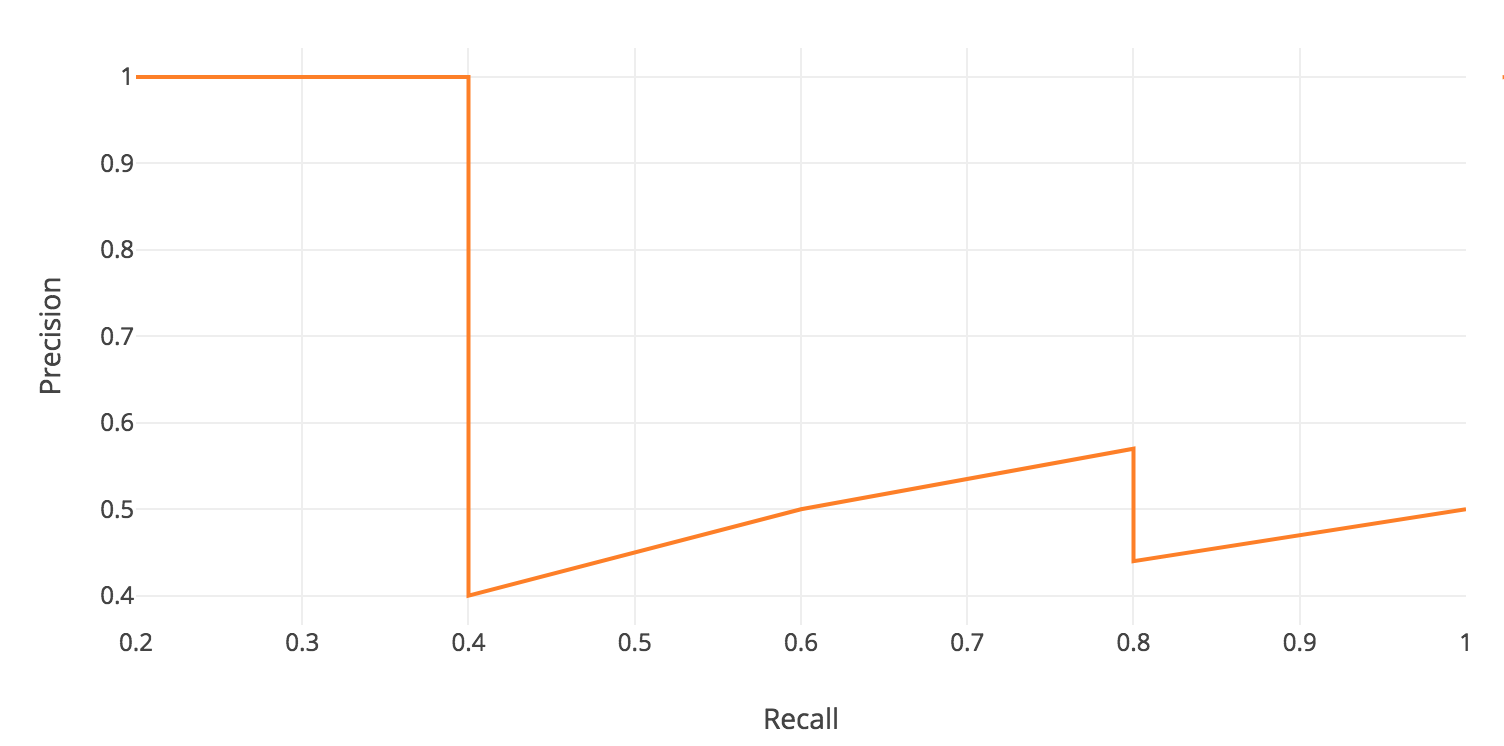
\includegraphics[width=\columnwidth]{imgs/pr_curve.png}
    \caption{Example of a precision-recall curve, where precision and recall were calculated for different \ac{IoU} thresholds and sorted and plotted by their recall values \cite{map_article}. The \ac{AP} is the area under the curve.}
    \label{fig:pr_curve}
\end{center}
\end{figure}

\subsubsection{Mean Average Precision (mAP)}

An extension of the \ac{AP} metric is the \ac{mAP}, which measures overall classification performance for all classes combined.
It is calculated as the mean of all classwise \acp{AP}, where $C$ is the number of classes (equation \ref{eq:map}).

\begin{equation}
    \text{mAP}(\text{AP}) = \frac{1}{C} \sum_{i=1}^C \text{AP}_i
    \label{eq:map}
\end{equation}

\subsubsection{Mean Intersection over Union (mIoU)}

\ac{mIoU} is a metric often used in segmentation tasks.
As the name suggests it measures the \ac{IoU} between the predicted mask and the ground truth mask.
Further, the mean of all \ac{IoU} values is calculated over the number of measured samples $N$ and results in the final \ac{mIoU} value (equation \ref{eq:miou}).

\begin{equation}
    mIoU = \frac{1}{N} \sum_{i=0}^{N} \text{IoU}_i
    \label{eq:miou}
\end{equation}
